% Chapter Template

\chapter{Human-Aware Robot Guide} % Main chapter title

\label{chapter:case_study} % Change X to a consecutive number; for referencing this chapter elsewhere, use \ref{ChapterX}

\lhead{Chapter 10. \emph{Robot Guide}} % Change X to a consecutive number; this is for the header on each page - perhaps a shortened title

In this chapter we present some applications of our system. First, in section~\ref{sec:case_study-spencer} presents a human aware robot guide. subsection~\ref{sec:spencer-intro} presents the subject and the motivations of our application. subsection~\ref{sec:spencer-robot_guide} shows how we adapted our architecture to scenario. subsection~\ref{sec:spencer-intention} introduces a new intention recognition algorithm developed for this task, based on environmental informaton. The scenario required a different approach to task planning than the one we developed, and we show our solution in subsection~\ref{sec:spencer-planning}. To guide humans, we developed a new collaborative planner, which is shown in subsection~\ref{sec:spencer-collaborative_guide_planner}. Finally, subsections \ref{sec:spencer-lab_experiments} and \ref{sec:spencer-airport} show our results in a laboratory and in a real environment.

\section{Introduction}
\label{sec:spencer-intro}
\subsection{Overview on the topic}
One interesting problem in human-robot interaction is developing robots able to guide humans, by offering a tour of attractions in an area or simply by helping to reach a destination.
A generic mobile robot platform should possess a vast set of skills, which includes advanced perception, motion planning, and task planning. These skills are not enough for a robot guide, which is deployed in highly dynamic human environments, and need to be complemented with human-aware behaviors.

%Examples
Different robot guides have been studied and developed, starting with pioneers like Rhino and Minerva \citep{thrun2000probabilistic}.  Few systems have actually been deployed for long period of time in human environments. Rackham \citep{clodic2006rackham}, a museum guide with human-aware behaviors, is an example of such system, and has been deployed in a science museum for several months.  Rackham's algorithm, like voice and face recognition, enables it to estabilish a form of relationship with his users, and to consider the task as a collaborative activity. For example, Rackham will stop if the user go away and wait for a period of time, resuming the task if it recognize the user coming back.
 Another example of robot guide was developed in \cite{bueno2011autonomous}, where the robot is integrated  in a smart museum environment, using virtual avatars with human-aware interfaces, associated to exhibitions, in order to convey information to users. 

 After these first experiments, several researchers have tried to focus on the social aspects of the problem, which are especially important if the robot needs to offer information. Studies like \cite{yousuf2012development,evers2014development} focus on how the robot should address humans, concentrating on spatial relationships and on how to convey information.  \cite{Jensen2005} present a robot guide able to convey emotions to user, by joining perceptual information with the internal state of the robot. 

Building and using mental models of users is important in these scenarios, particularly if we are developing a proactive robot, which approaches people in order to offer its services, while monitoring their level of interest in the interaction.  In \cite{rashed2015toward}, a robot guide is able to infer people's intention by studying their trajectories. The authors conducted experiments in a museum, managing to classify user trajectories in three categories: users interesting in looking at a collection of painting, users looking for a particular painting, users visiting the museum by chance. By recognizing the trajectory of a user the robot infers if he could be interesting in a guided tour.

Recently, there has been emphasis on robot navigation algorithms that reason about human beings in the environment differently from other static or dynamic obstacles. Starting from proxemics, researchers have investigated explicit social signals, based on human-posture and the affordances of the environment, to improve the legibility of the robot's motions. For a detailed discussion on human-aware navigation algorithms we refer the readers to \cite{kruse2013human,rios-ijsr-2014}. Human-aware navigation in a museum situation was studied in \cite{samejima2015building}, where the authors build environmental maps, which include information learnt from human trajectories and postures, in order to plan safe paths that do not disturb humans present in the area. 

The robot guide scenario can become more complex if we consider not only single humans, but groups. Humans, in fact, tend to naturally form groups, which can be classified in different types, based on their size, on their level of cohesion, on their duration, and other factors \citep{forsyth2009group}.  Studying group formations is a complex problem, since the robot must be able to detect humans, which can be occluded in populated environments; and to model their social interactions, which can be ambiguous. One of the most powerful and expressive social cues is distance, used in different works to track social relationship, like \cite{luber2013multi}. 

\subsection{Motivations}
We believe that most robot guide systems are focusing on the social aspects of the problem, and on human-aware navigation, without fully considering the fundamental aspects of joint actions. Guiding is a collaborative task, where the robot does not need only to reach a destination, but also to ensure that its followers reach it, while providing a socially acceptable experience to them. In order to achieve this goal, the robot needs to constantly monitor its users, to adapt to their behaviors and to be ready to proactively help them.

We applied our system to this problem, creating a human-aware robot guide which is able to lead a group of people to a destination. More particularly, the originality of our approach is that the robot is able to show both adaptive and a proactive behaviors. The robot will try, while guiding, to select a speed that pleases its users, when adapting, or to propose a new speed, using environmental and task related stimulus. Finally, our system will proactively try to engage members of the group if it detects they need assistance. 

\section{Building a Robot Guide}
\label{sec:spencer-robot_guide}
In order to adapt our system to the robot guide scenario we had to enhance several modules, as shown in figure \ref{fig:spencer-architecture}: 
\begin{itemize}
\item The user is able to interact with the robot by using a tactile interface on its front. Partners in the project developed an interface that connects this tablet to requests for the robot.
\item In this scenario we are not really interested in the intention recognition skills that we developed in chapter~\ref{chapter:situation_assessment}. In an airport there are no complex sequence of actions that humans need to perform and we will evaluate users' intentions by their trajectories and the surrounding environment. We developed an Environment-Based Intention Situation Assessment module to enhance our Situation Assessment layer, presented in section \ref{sec:spencer-intention}.  
\item Similarly, task planning and plan management is quite simple in this scenario. The robot will mostly vary its paths in the environment, using similar plans. We developed an A*-based task planner, which is able to find a path in a semantic map, to guide users to their destination, presented in section~\ref{sec:spencer-planning}. The Plan Management layer will receive this plan and communicate with the Task Execution layer to move the robot toward the goal.
\item The main work, in this application, has been creating a Collaborative Planner to guide users in a human-aware way. Using this planner, our robot is able to adapt itself to users' actions, or to proactively propose new behaviors. This planner is presented in section~\ref{sec:spencer-collaborative_guide_planner}.
\end{itemize} 

\begin{figure}[ht!]
	\centering
	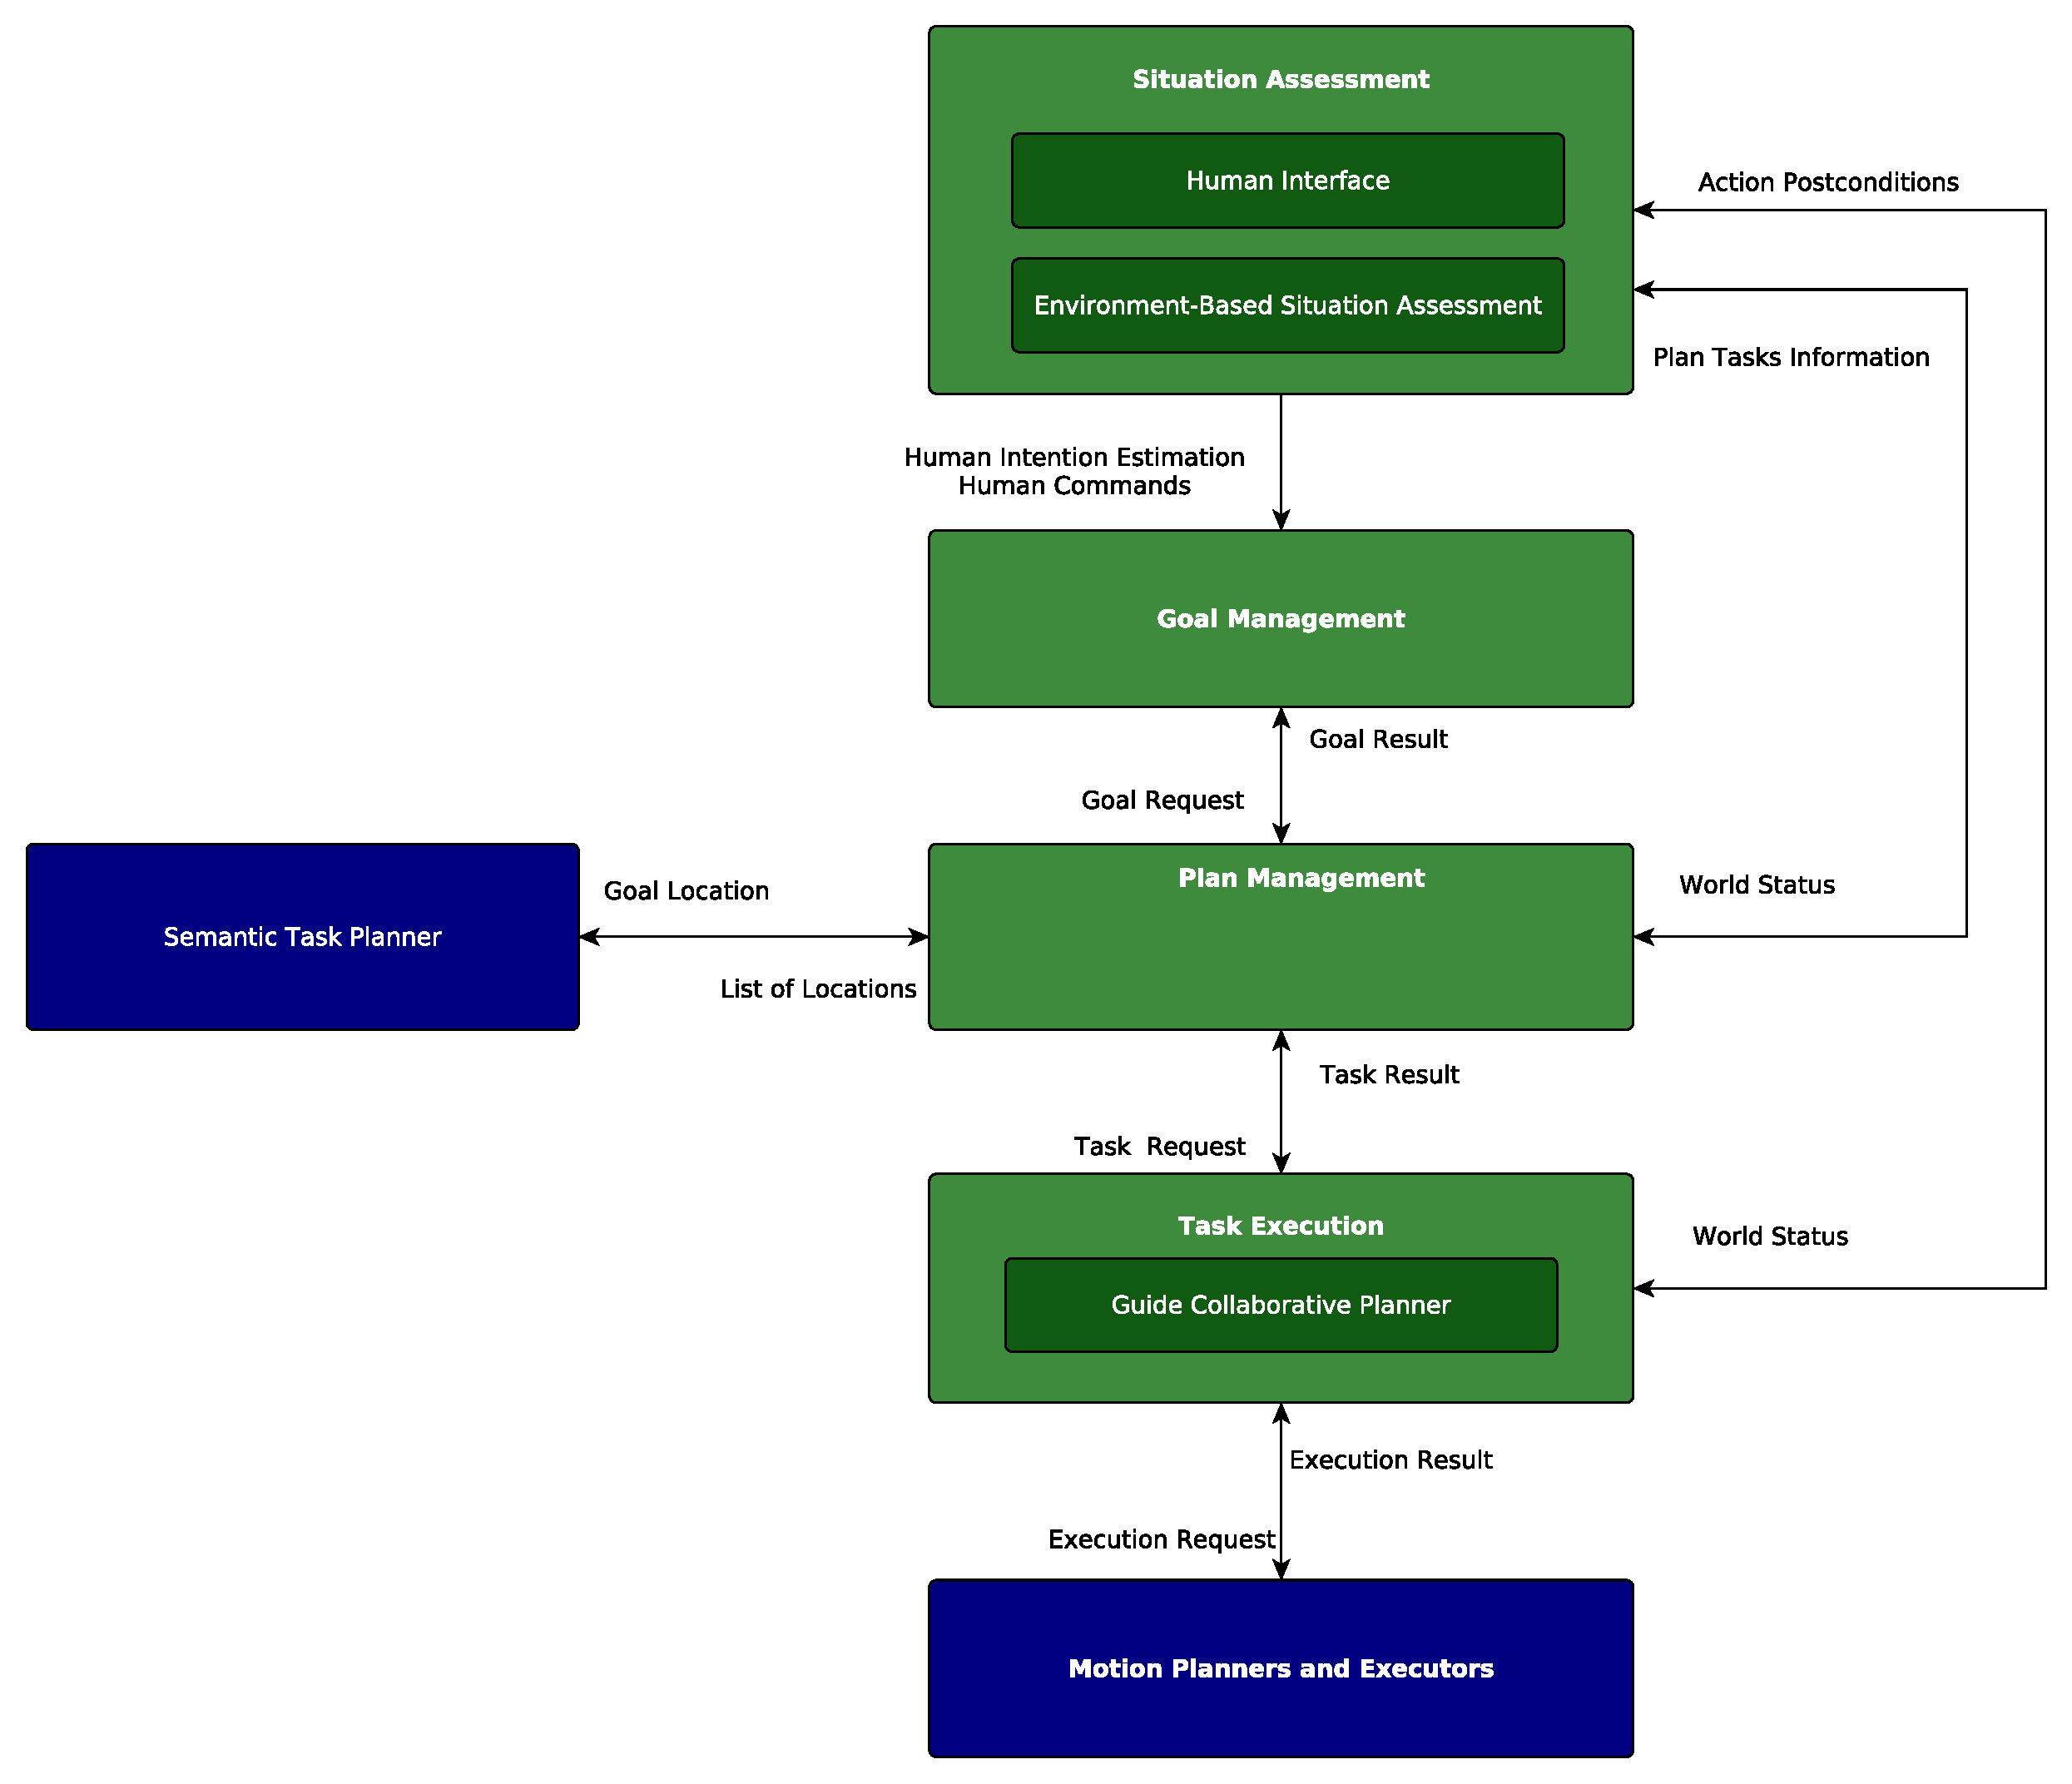
\includegraphics[scale=0.38]{img/case_study/spencer/architecture.pdf}
	\caption[Robot guide architecture]{This image shows the main layers of our architecture, represented as dark green rectangles, as shown in chapter~\ref{system_overview}. In each layer, represented as light green rectangles, we show the modules that we modified or introduced in the robot guide scenario. Blue rectangles represent external modules. The Semantic Task Planner was specifically created for this scenario.}
	\label{fig:spencer-architecture}
\end{figure}

The system has been tested with different configurations, in laboratory experiments and in the Schipol airport, presented in chapter~\ref{chapter:spencer_results}. 

Parts of this section were presented in \cite{fiore2015adaptive}.

\section{Environment-Based Situation Assessment}
\label{sec:spencer-intention}
There are many situations where, to properly reason on humans, we should link their movements and actions to the current environment. Imagine for example the case where we see a person oriented toward a screen. In an airport, we could infer from this observation that the person is looking at the screen, and perhaps in need of information. 

We introduced, in the Situation Assessment layer, the ability able to create activity areas in the environment and link them to different kind of computations. An activity area is a polygonal or circular area, which can be fixed or linked and updated with an entity's (object, human or robot) position. We studied and experimented three activity areas:

\begin{itemize}
\item Information Screen Area. This area, shown in figure \ref{fig:spencer-screen_area} is linked to information screens present in the environment. Using this information, the robot can recognize that humans are looking at the screen, and  start a proactive behavior, like approaching to offering help or information.
\item Touristic Point Area. These areas are linked to interesting sights and attractions in the environment. We can imagine, for example, to associate these areas to paintings, statues, or even rooms in a museum. Knowing that a human is in a touristic point area, and looking at an attraction, the robot could approach the human and tell him some interesting information about it.
\end{itemize}

\begin{figure}[ht!]
	\centering
	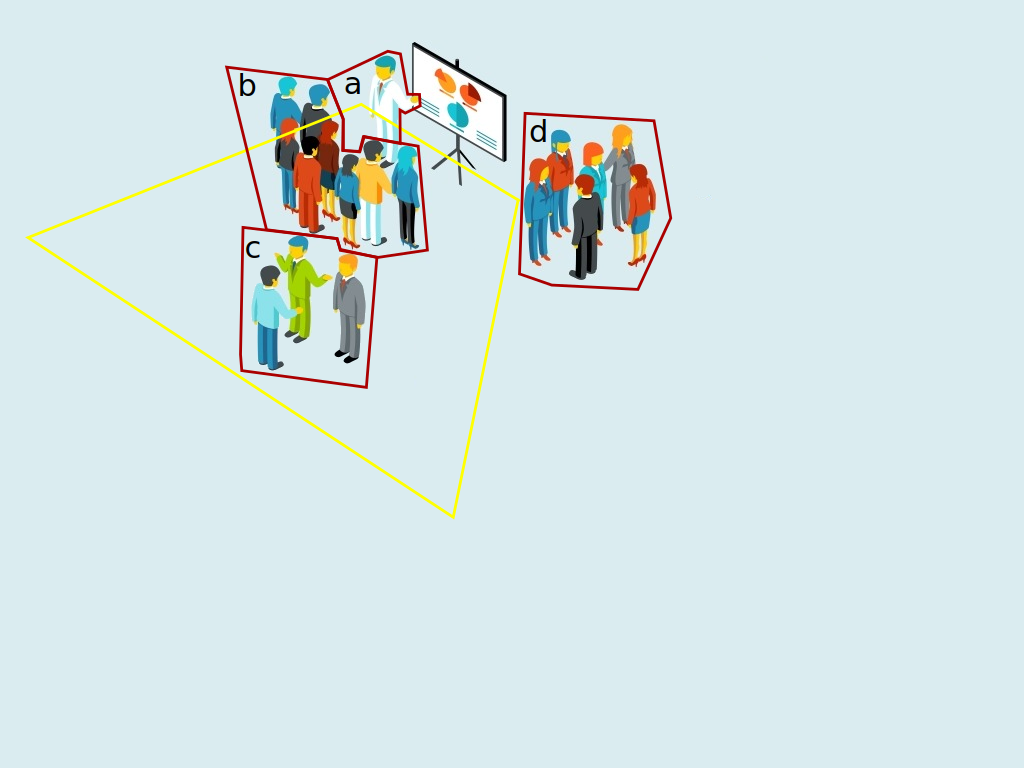
\includegraphics[scale=0.45]{img/case_study/spencer/environment_intention.pdf}
	\caption[Environment-Based Situation Assessment]{The Information Screen area used for environment-based intention recognition. The yellow polygon represents an area linked to the screen in the figure. Red polygons represent groups of person in the area. The person in group \textit{a} is in the screen area, but the robot will infer that he is not looking at the screen, since he is oriented in another direction. The persons in group \textit{b} are in the screen area and oriented toward the screen, so the robot infers that they are looking at it. The persons in group \textit{c} are not looking at the screen since they are either oriented in another direction or outside its area.}
	\label{fig:spencer-screen_area}
\end{figure}

\section{Task and Motion Planning Problems}
\label{sec:spencer-planning}
To guide people in environments like museum or airports, the robot will need to navigate very large areas, which are often too big to efficiently perform motion planning. A solution to this problem is reducing the size of the area where the motion planner will compute its paths, splitting the navigation problem in a list of sub goals. The problem, with this approach,  is choosing the correct list of sub-goals to reach the final position.  To deal with this issue we implemented an A*-based task planner, which will choose a high-level path to be followed by the robot from a semantic map. This map is a hand-crafted graph, composed by different nodes, that represent parts of the environemt (corridors, elevator entrances, gates, etc.). Each node will be linked to a point in the real world. This task planner will, so, produce a list of coordinates usable by the motion planning layer. 

\begin{figure}[ht!]
	\centering
	\includegraphics[scale=0.45]{img/case_study/spencer/ShengenTaskPlanner.png}
	\caption[Robot Guide Plan]{An example of plan computed in the robot guide scenario. The circles represent nodes in the semantic map. The purple node is the starting node of the plan. The red node is the goal. The green nodes represent intermediate nodes in the plan.}
	\label{fig:spencer-semantic_plan}
\end{figure}


A first way to manage this kind of plan is simply travelling to each calculated point, sending a goal to the motion planner for the next point every time the robot reaches its sub-destination. The problem with this approach is that the path followed by the robot might be very inefficient and not look natural.

Our solution was using a rolling window approach, shown in figure~\ref{fig:spencer-rolling_window}, where the motion planner will compute paths on a grid map centered on the robot, which will be updated with its position. In this way, the robot will send the next sub-goal in the calculated plan as soon as it is present in the rolling window, without waiting to reach the previous sub-goal. It is very important, with this approach to carefully select the nodes in the semantic maps so that the rolling window will contain at least two semantic nodes. If not, the motion planner would have to plan a path to a goal outside its grid map, which would generate an error.


\begin{figure}[ht!]
	\centering
	\includegraphics[]{img/case_study/spencer/rolling_window.pdf}
	\caption[Rolling window]{This figure shows the rolling window approach. The motion planner will compute robot paths in the grid represented by the yellow area, which is always centered on the robot. The red line and the red dots represent the sequence of goals calculated by the task planners. Each goal from this path is sent to the motion planner as soon as it is inside the window. The robot path does not pass through the closest node, since there is a further one in the rolling window.}
	\label{fig:spencer-rolling_window}
\end{figure}

\section{Collaborative Guide Planner }
\label{sec:spencer-collaborative_guide_planner}

We developed a new collaborative planner to guide users to a destination. The planner is organized as a hierarchic MOMDP, as shown in figure \ref{fig:spencer-guide_planner} and is composed by several models:
\begin{itemize}
\item Guide Group Model. The main MOMDP of the hierarchy, responsible of choosing the main action performed by the robot.
\item Speed Adaptation Model. This model chooses if the robot should accelerate, decelerate, or keep the current speed.
\item Suspend Model. This module chooses which actions to execute when the users has stopped following.
\end{itemize}



\begin{figure}[ht!]
	\centering
	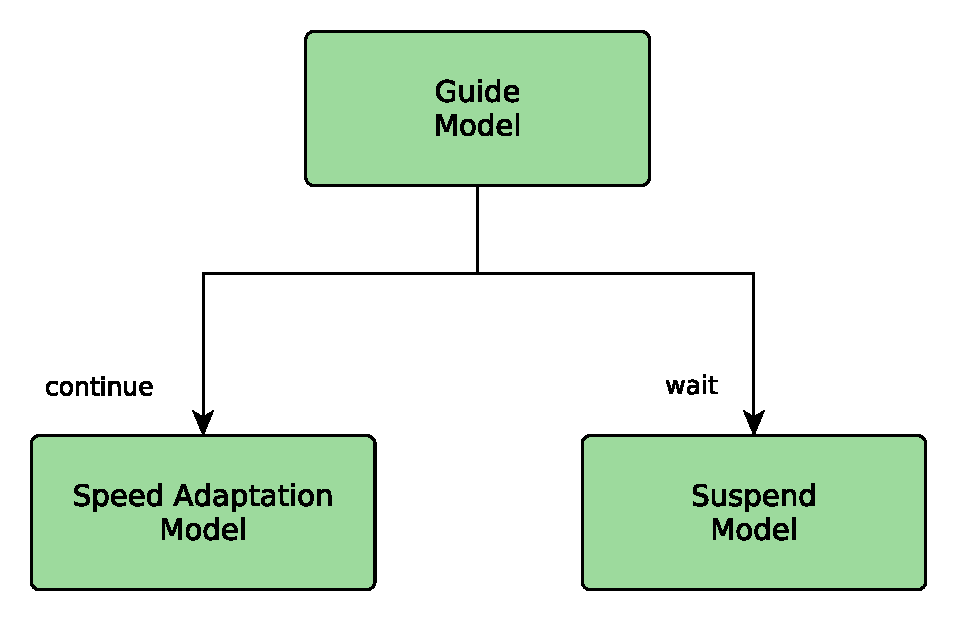
\includegraphics[scale=0.45]{img/case_study/spencer/guide_planner.pdf}
	\caption[Collaborative planner for guiding]{This figure shows the hierarchical MOMDP collaborative planner use to guide a Group. The arrows show the macro-actions of the root of the hierarchy, leading to sub MOMDPs.}
	\label{fig:spencer-guide_planner}
\end{figure}

\section{Representing a group}
Our system has been built with the assumption that the robot would navigate in a crowded environment, where its followers could be often occluded. In addition, after speaking with our partners, we understood that the perception components would not be able to maintain a stable identifier for members of the groups, meaning that the robot would not be able to realiably understand if a group of users is following it. We tried to maintain a good balance between accuracy, trying to guide effective users and not people whose which are going in the same direction as the robot, and robustness, copying with unreliable perception.

We built our collaborative planner following these ideas:
\begin{itemize}
\item The robot will record a list $g$ composed by the identifiers of the group at the start of the scenario. During this scenario, it will maintain a list $f$, composed by users that are still tracked whose identifier is in $g$, and another list $o$, composed by all the tracked people whose distance from the robot is less than a costant $d$. 
\item As long as $f$ is not empty, the robot will choose a \textit{best} follower $b$ from this list, and try to guide him, using the collaborative planner. The \textit{best} follower is chosen by considering the user whose behavior is the most consistent with the robot, by taking into account the speed, distance and orientation of the user.
\item If $f$ is empty, but $o$ is not, the robot will choose a \textit{best} follower $b$ from $o$, and try to guide him, using the collaborative planners.
\item If  both $f$ and $o$ are empty, the robot will abandon the task.
\end{itemize}

Our idea is considering that the robot's followers will \textit{act as a group}, staying together as much as they can. The robot will try to guide members of the group, but if it has lost tracking of all of them, and there is still somebody behind it which is acting in a consistent way with the guiding task, it will think that its users are still following it, but their identifiers have changed in the perception layer.


\subsection{Guiding a User}
The main problem of the robot is choosing if it should still guide the group, suspend temporarily the task, or abandon it. The Guide Model is the root MOMDP of our architecture and will make this decision, based on three main variables: 
\begin{itemize}
\item The status of advancement of the task. This variable, whose values are \textit{\{not\_completed, completed\}}, is set by the Action Executor module, in the Execution Management layer, depending on the current advancement of the task. The variable will be set as $not\_completed$ until the robot as reached the final destination in the plan. 
\item The quality of commitment of the group. This variable, whose values are \textit{\{not\_engaged, engaged, not\_interested\}}, is hidden, estimated from observations produced by the Situation Assessment layer. The observations used are: the distance of the user from the robot, its variation, the orientation of the user in respect of the  robot, and if the user is currently moving or still. We expect engaged users to have a behavior that is coherent with the task, moving to follow the robot and taking a similar path. Users are considered not engaged when they stop following, perhaps even disappearing from the robot's sight. Finally, we infer that users are not interested in following the robot if they have been \textit{not\_engaged}  for too long.
\item A timer. This variable can assume the values \textit{\{not\_expired, expired\}}. When a user is detected as $not\_engaged$, the Action Executor starts a timer. When this timer expires, the value of this variable is set accordingly.
\end{itemize}

The Guide Model can execute the following actions:
\begin{itemize}
\item $Continue$. A macro-action, which leads to the Speed Adaptation Model.
\item $Wait$. A macro-action, which leads to the Suspend Model.
\item $Abandon$. Signals the Action Executor to abandon the current task.
\end{itemize}

\subsection{Adapting the Robot's Speed}
We believe that to be socially acceptable, the robot should adapt its speed to his follower. By setting its own pace at the start of the scenario the robot  would risk of being too slow, annoying users, or too fast, which would lead the robot to constantly stop to wait for users, producing an awkward behavior. Adapting to users might not be enough in some tasks, and, depending on the situation, the robot might desire to influence the behavior of its follower, to respect social rules or to accomplish its task in a more efficient way. Its important to find a balance between these two behaviors, which is the goal of the Speed Adaptation Module. 

To adapt to the speed of the group, the robot defines a desired range of distances $[dr_1,dr_2]$ from the best follower $b$. The distance of $b$ from the robot, $d(b,r)$ will influence the chosen action:
\begin{itemize}
\item if $d(b,r)>dr_2$  the model will influence the robot to \textit{decelerate}.
\item if $d(b,r)<dr_1$ the model will influence the robot to \textit{accelerate}.
\item if $dr_1<d(b,r)<dr_2$ the model will influence the robot to maintain its current speed.
\end{itemize} 

In our study, $dr_1$ and $dr_2$ were predefined values, but they could be learnt and adapted to the users during the task, since different people could prefer following the robot at different distances and positions.

The robot should also not constantly change speed, in order to give time to users to adapt to its new chosen speed, and so we defined a temporal threshold in which we do not allow the robot to repeat an \textit{accelerate} or \textit{decelerate} action.

We studied two different situations where the robot can proactively try to influence the speed of the group.
\begin{itemize}
\item There is a time limit to reach the destination. In this case the robot must balance the desire to satisfy the group with the task urgency. Different situations will require different policies. For example, in an airport scenario, the robot could prioritize arriving on time, warning users if their speed would render the goal not achievable, while in other situations the robot could try to arrive in time but still avoid to adopt speeds that are uncomfortable for the group.
\item The rules of the current environment limit the robot's speed. In this case the robot will avoid accelerating over a set speed even if it detects that its current velocity is considered too slow for the group. For example, the robot could be navigating in a construction zone.
\end{itemize}

\subsection{Suspending the task}
In some situation, the robot needs to suspend the task, because the group has stopped following it. In this case, the robot should estimate if this suspension of the collaborative scenario is temporary or permanent, and in the latter case abandon the task. We estimate this information using the Suspend Model and the activity areas from Situation Assessment. We link activity areas to the maximum time we expect that the group will be involved in the linked activity, and with a set of proactive actions that the robot can choose to execute.

In our work, we investigated a single possible proactive behavior: giving information. In this case, if we detect that one or more  members
of the group has stopped following because it is looking at a touristic sight, or at an information screen, the robot can try to engage him and offer related information. At the moment, we just propose a simple routine-based framework for this behavior, and plan to further study it in the future. We believe that the solution of this problem could be rich, and that the robot should estimate the reaction of the group during the execution of its proactive behavior, in order to be able to interrupt if the group does not want to be helped or to resume the original task if they are satisfied by the robot's actions.

We do not want the robot to be inactive for a long time  waiting for the group. If there is a small amount of time to reach the destination, or the group is engaged in the activity for a longer period of time than the one predicted, or the robot can not estimate the reason why the group stopped following, the Suspend Model can issue a warning action, and eventually abandon the task if the group does not start following it again.



